% !TEX root = ../../semexp-thesis.tex

\section{Semantic Object Interfaces for Exploratory Programming}
\label{sec:design/agent}

\begin{figure}
	\centering
	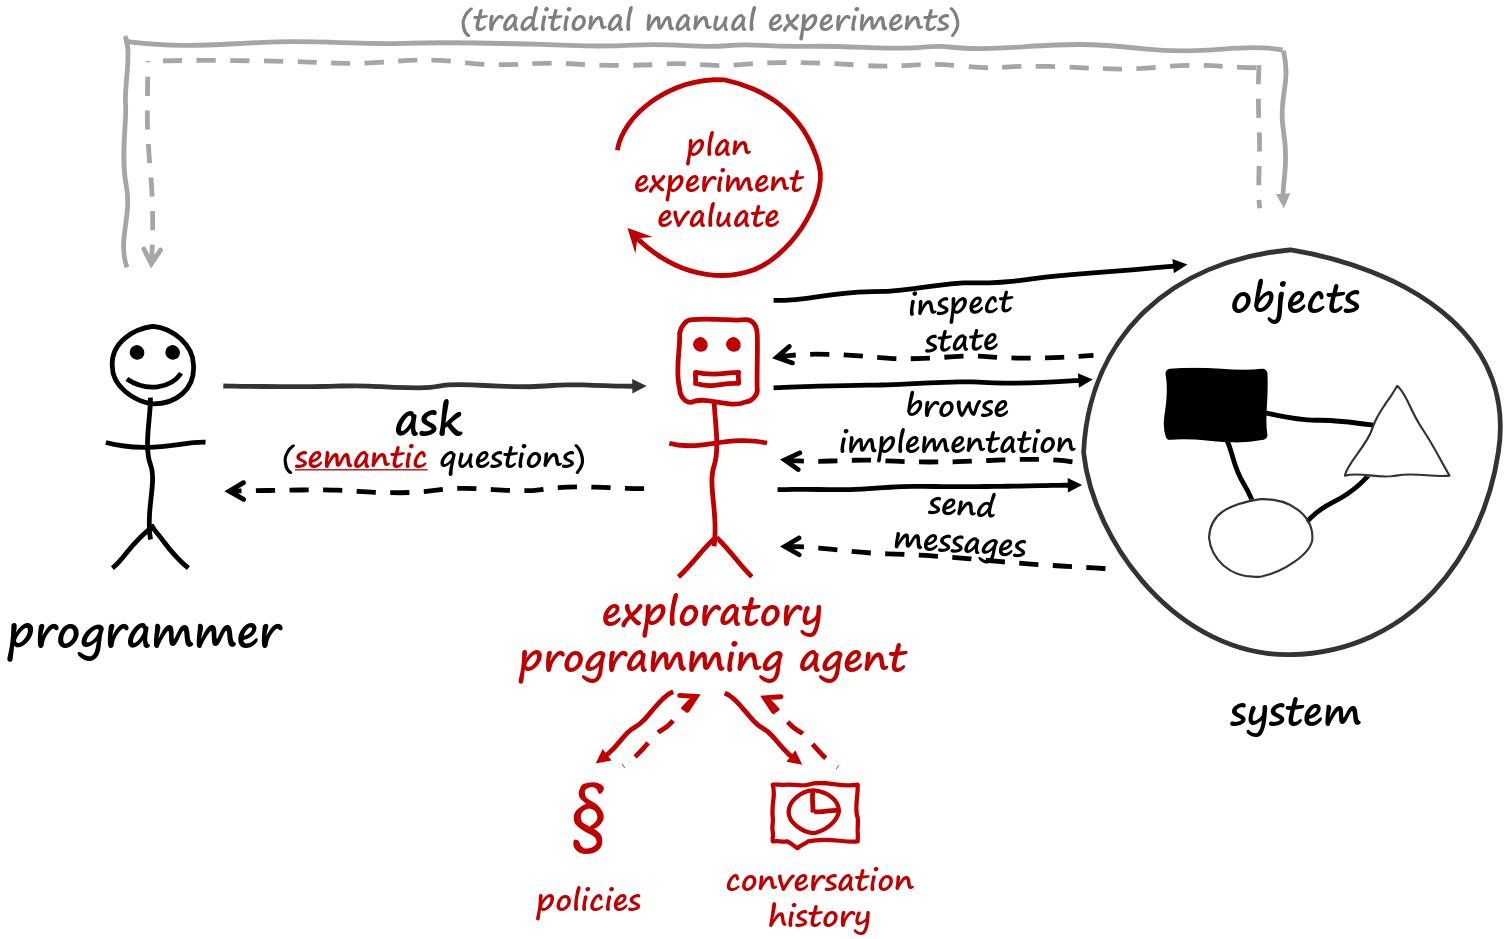
\includegraphics[width=.9\textwidth]{03_agent/framework.png}
	% todo: update figure: use revised vocabulary and darker red. update red reference in this and other captions.
	\caption[Our approach of semantic object interfaces for semantic exploratory programming systems.]{
		Our approach of semantic object interfaces for semantic exploratory programming systems.
		The programmer expresses high-level, contextual, and often natural-language questions about an object to the interface and receives answers on the same abstraction level.
		Internally, an \emph{exploratory programming agent} (\textcolor{red}{red}) translates these questions and interacts with the system to perform low-level experiments.
	}
	\label{fig:design/agent/framework}
\end{figure}

To delegate parts of the research process to the exploratory programming system, we construct an \emph{exploratory programming agent}, which uses a generative LLM for planning, generating experiments, and communicating with the programmer in natural language.
To connect the agent with the programming system, we propose the design of an \emph{semantic object interface} that describes the communication between the programmer, the agent, and the system~(\cref{fig:design/agent/framework})~\cite{thiede2024talking}.
Our approach follows the object-oriented paradigm of many programming systems in that semantic interfaces focus on a single object from the running system.
Thus, semantic object interfaces resemble traditional message sending to objects, and programmers can interact with objects via the agent by the means of natural-language and semantic questions.

As part of this framework, the agent takes high-level and context-dependent \emph{semantic} questions from the programmer and translates them into low-level technical experiments to answer the questions.
Our framework comprises three fundamental actors:

\begin{description}[noextralabelsep]
	\item[The programmer] conducts a larger exploratory research process, from which different questions arise.
	The programmer asks such questions about an object in a system and expects answers on a similar level of abstraction.
	These questions are \emph{semantic} and conceptual, meaning that they are expressed in the programmer's mental model and vocabulary, typically formulated in an informal and natural-language style, and often depend on the context of previous questions and answers.

	\item[The object] is any object in the system, for example a particular domain object, a code object (such as a class or method), or an artifact from the programming system (such as a call graph, a benchmark, or a program trace).
	It is usually part of an \emph{object graph} which embeds it into a larger context of the system.
	It is also linked to any form of \emph{implementation} that describes the object's behavior through further objects; this may manifest as code, tests, or other kinds of specifications such as contracts.

	Objects can be accessed either by sending them \emph{messages} (which in many languages is also referred to as \emph{invoking methods}) or through \emph{reflection interfaces} that expose their internal state, implementation, or location in the object graph.

	\item[The exploratory programming agent] is an intelligent mediator between the programmer and the object in the system that translates conceptual questions from the programmer into interactions with the system and responds to the programmer.

	Internally, the agent conducts research processes autonomusly: it interprets the programmer's question, develops a plan, designs and executes experiments, evaluates their results, and iterates as necessary, before it generates a final answer to the questions and returns it to the programmer.

	The agent uses two resources: a set of \emph{policies} and a \emph{conversation history}.
	First, \emph{policies} define the abstract agent behavior, such as the types and frequency of experiments or the format of answers.
	Second, the \emph{conversation history} contains past communications with the programmer as well as experiments from the current conversation.
	It serves as a context for handling subsequent requests.
	Thus, the programmer does not need to restate their mental model and intentions in every question but grows a shared vocabulary and knowledge with the agent as the conversation evolves.
\end{description}

This framework allows programmers to ask arbitrary questions about objects in a system that can reference two different aspects:

\begin{description}[noextralabelsep]
	\item[Functional questions] (or ``what'' questions) refer to the state of objects and the domain instance they represent.
	They typically display inquiries that are or could be covered by regular (analytical) system features or objects' behavior.

	For example, in a sales system, typical functional questions could be ``How many customers are there?'', ``Which product in this category has generated the highest profit in the last quarter?'', or ``What is the age distribution of weekend customers?''.

	\item[Epistemic questions] (or ``how'' questions) refer to the behavior of objects, the concepts of the domain, and the implementation thereof.
	They are intended to explore the capabilities of a system, understand the technical foundations, or ideate and prototype new applications.

	For example, in a sales system, epistemic questions could include ``What information do we store about customers?'', ``How is the tagging system for products modeled like?'', or ``How can we analyze the shopping behavior of customers?''.

	Note that given the uniform object model of many programming systems, epistemic questions about a domain object equal functional questions about a code object from the implementation of the domain; however, the former perspective provides additional context about the system through a concrete example.
\end{description}

To answer these questions, the agent conducts experiments by utilizing three types of interfaces that are offered by the traditional programming system:

\begin{description}[noextralabelsep]
	\item[State inspection] allows the internal state of objects to be explored, for instance, by looking up a variable or enumerating all properties.
	\item[Implementation browsing] explores the specified behavior of objects\linebreak{}through their protocols, implementation, and documentation.
	Protocols refer to the set of messages an object understands.
	Implementation includes the source code of objects or classes, but also their integration within the global system through call graphs or related concepts (e.g., senders or program traces), which can be a valuable source of context about possible usages and compositions of objects and their behavior.
	Documentation can be provided through comments, examples, or alternative system descriptions.

	Following the singularity of objects and meta objects noted above, implementation browsing of domain objects equals state inspection of their classes, but is associated with a different connotation by adhering to the context of the original object.
	For example, using symbolic execution methods, both the state and effective behavior of objects can explored at once.
	\item[Message sending] constitutes the regular usage of objects to activate their behavior and does not require reflective methods.
\end{description}

Note that the agent generally does not require any manual preparation for specific systems from domain experts or programmers but will learn about the system on its own.
Thus, even to answer simple functional questions, the agent needs to internally ask and answer epistemic questions to understand the system and domain concepts.
Analogously, every message send to an unknown system is preceded by browsing its implementation, through which the agent discovers the relevant protocols and messages to use.

\begin{example}
	A programmer asks ``Which product has generated the highest profit?'' about a selected shop object.
	In response, the agent first executes a series of experiments by browsing the shop's implementation to explore several messages, classes, and their documentation related to the concepts ``product'' and ``profit'' to understand what these concepts mean and how they are represented in the system.
	After identifying relevant messages such as \code{Shop>>orders}, \code{Order>>productItems}, and \code{Product>>price}, it plans how to combine this information to compute the most profitable product and runs a script that queries the system for this information as another experiment.
	Finally, the agent evaluate the results of this experiment and returns an answer in natural language to the programmer.
\end{example}

Thus, semantic object interfaces allow programmers to delegate parts of their research process to the programming system by expressing conceptual questions, letting an exploratory programming agent research them autonomously and conduct low-level experiments, and receiving conceptual answers in natural language.
